% Options for packages loaded elsewhere
\PassOptionsToPackage{unicode}{hyperref}
\PassOptionsToPackage{hyphens}{url}
\documentclass[
]{article}
\usepackage{xcolor}
\usepackage[margin=1in]{geometry}
\usepackage{amsmath,amssymb}
\setcounter{secnumdepth}{5}
\usepackage{iftex}
\ifPDFTeX
  \usepackage[T1]{fontenc}
  \usepackage[utf8]{inputenc}
  \usepackage{textcomp} % provide euro and other symbols
\else % if luatex or xetex
  \usepackage{unicode-math} % this also loads fontspec
  \defaultfontfeatures{Scale=MatchLowercase}
  \defaultfontfeatures[\rmfamily]{Ligatures=TeX,Scale=1}
\fi
\usepackage{lmodern}
\ifPDFTeX\else
  % xetex/luatex font selection
\fi
% Use upquote if available, for straight quotes in verbatim environments
\IfFileExists{upquote.sty}{\usepackage{upquote}}{}
\IfFileExists{microtype.sty}{% use microtype if available
  \usepackage[]{microtype}
  \UseMicrotypeSet[protrusion]{basicmath} % disable protrusion for tt fonts
}{}
\makeatletter
\@ifundefined{KOMAClassName}{% if non-KOMA class
  \IfFileExists{parskip.sty}{%
    \usepackage{parskip}
  }{% else
    \setlength{\parindent}{0pt}
    \setlength{\parskip}{6pt plus 2pt minus 1pt}}
}{% if KOMA class
  \KOMAoptions{parskip=half}}
\makeatother
\usepackage{longtable,booktabs,array}
\usepackage{calc} % for calculating minipage widths
% Correct order of tables after \paragraph or \subparagraph
\usepackage{etoolbox}
\makeatletter
\patchcmd\longtable{\par}{\if@noskipsec\mbox{}\fi\par}{}{}
\makeatother
% Allow footnotes in longtable head/foot
\IfFileExists{footnotehyper.sty}{\usepackage{footnotehyper}}{\usepackage{footnote}}
\makesavenoteenv{longtable}
\usepackage{graphicx}
\makeatletter
\newsavebox\pandoc@box
\newcommand*\pandocbounded[1]{% scales image to fit in text height/width
  \sbox\pandoc@box{#1}%
  \Gscale@div\@tempa{\textheight}{\dimexpr\ht\pandoc@box+\dp\pandoc@box\relax}%
  \Gscale@div\@tempb{\linewidth}{\wd\pandoc@box}%
  \ifdim\@tempb\p@<\@tempa\p@\let\@tempa\@tempb\fi% select the smaller of both
  \ifdim\@tempa\p@<\p@\scalebox{\@tempa}{\usebox\pandoc@box}%
  \else\usebox{\pandoc@box}%
  \fi%
}
% Set default figure placement to htbp
\def\fps@figure{htbp}
\makeatother
\setlength{\emergencystretch}{3em} % prevent overfull lines
\providecommand{\tightlist}{%
  \setlength{\itemsep}{0pt}\setlength{\parskip}{0pt}}
\usepackage[]{natbib}
\bibliographystyle{plainnat}
\usepackage{booktabs}
\usepackage{longtable}
\usepackage{array}
\usepackage{multirow}
\usepackage{wrapfig}
\usepackage{float}
\usepackage{colortbl}
\usepackage{pdflscape}
\usepackage{tabu}
\usepackage{threeparttable}
\usepackage{threeparttablex}
\usepackage[normalem]{ulem}
\usepackage{makecell}
\usepackage{xcolor}
\usepackage{bookmark}
\IfFileExists{xurl.sty}{\usepackage{xurl}}{} % add URL line breaks if available
\urlstyle{same}
\hypersetup{
  pdftitle={pokemon-statistical-analysis},
  pdfauthor={Angelo Freda},
  hidelinks,
  pdfcreator={LaTeX via pandoc}}

\title{pokemon-statistical-analysis}
\author{Angelo Freda}
\date{2026-03-01}

\begin{document}
\maketitle

{
\setcounter{tocdepth}{2}
\tableofcontents
}
\subsection{Objetivos Específicos}
\begin{itemize}
  \item{Poder Legendario: ¿Son realmente más fuertes los Pokémon legendarios en comparación con los comunes?}
  \item{Análisis por Tipo: Determinar qué tipo posee las mejores estadísticas en promedio.}
  \item{Pseudo-legendarios: Evaluar si si son realmente competitivos.}
  \item{Grupos de Huevo (Egg Groups): Analizar si influye el Egg group en nivel de combate.}
  \item{Evolución Generacional: Observar la Evolucion del poder por generación a lo largo de las generaciones.}
\end{itemize}

\section{Comparacion estadistica de los legendarios y los no los no
lejendarios.}\label{comparacion-estadistica-de-los-legendarios-y-los-no-los-no-lejendarios.}

\begin{table}[!h]
\centering
\caption{\label{tab:unnamed-chunk-1}Primeras 10 observaciones de Los Legendarios}
\centering
\resizebox{\ifdim\width>\linewidth\linewidth\else\width\fi}{!}{
\begin{tabular}[t]{cccccc}
\toprule
\cellcolor[HTML]{D7261E}{\textcolor{white}{\textbf{Name}}} & \cellcolor[HTML]{D7261E}{\textcolor{white}{\textbf{Type\_1}}} & \cellcolor[HTML]{D7261E}{\textcolor{white}{\textbf{Total\_Stats}}} & \cellcolor[HTML]{D7261E}{\textcolor{white}{\textbf{HP}}} & \cellcolor[HTML]{D7261E}{\textcolor{white}{\textbf{Attack}}} & \cellcolor[HTML]{D7261E}{\textcolor{white}{\textbf{Defense}}}\\
\midrule
\cellcolor{gray!10}{Articuno} & \cellcolor{gray!10}{Ice} & \cellcolor{gray!10}{580} & \cellcolor{gray!10}{90} & \cellcolor{gray!10}{85} & \cellcolor{gray!10}{100}\\
Zapdos & Electric & 580 & 90 & 90 & 85\\
\cellcolor{gray!10}{Moltres} & \cellcolor{gray!10}{Fire} & \cellcolor{gray!10}{580} & \cellcolor{gray!10}{90} & \cellcolor{gray!10}{100} & \cellcolor{gray!10}{90}\\
Mewtwo & Psychic & 680 & 106 & 110 & 90\\
\cellcolor{gray!10}{Raikou} & \cellcolor{gray!10}{Electric} & \cellcolor{gray!10}{580} & \cellcolor{gray!10}{90} & \cellcolor{gray!10}{85} & \cellcolor{gray!10}{75}\\
\addlinespace
Entei & Fire & 580 & 115 & 115 & 85\\
\cellcolor{gray!10}{Suicune} & \cellcolor{gray!10}{Water} & \cellcolor{gray!10}{580} & \cellcolor{gray!10}{100} & \cellcolor{gray!10}{75} & \cellcolor{gray!10}{115}\\
Lugia & Psychic & 680 & 106 & 90 & 130\\
\cellcolor{gray!10}{Ho-oh} & \cellcolor{gray!10}{Fire} & \cellcolor{gray!10}{680} & \cellcolor{gray!10}{106} & \cellcolor{gray!10}{130} & \cellcolor{gray!10}{90}\\
Regirock & Rock & 580 & 80 & 100 & 200\\
\bottomrule
\end{tabular}}
\end{table}
\begin{table}[!h]
\centering
\caption{\label{tab:unnamed-chunk-2}Primeras 10 observaciones de Los Legendarios}
\centering
\resizebox{\ifdim\width>\linewidth\linewidth\else\width\fi}{!}{
\begin{tabular}[t]{cccccc}
\toprule
\cellcolor[HTML]{0073C2}{\textcolor{white}{\textbf{Name}}} & \cellcolor[HTML]{0073C2}{\textcolor{white}{\textbf{Type\_1}}} & \cellcolor[HTML]{0073C2}{\textcolor{white}{\textbf{Total\_Stats}}} & \cellcolor[HTML]{0073C2}{\textcolor{white}{\textbf{HP}}} & \cellcolor[HTML]{0073C2}{\textcolor{white}{\textbf{Attack}}} & \cellcolor[HTML]{0073C2}{\textcolor{white}{\textbf{Defense}}}\\
\midrule
\cellcolor{gray!10}{Bulbasaur} & \cellcolor{gray!10}{Grass} & \cellcolor{gray!10}{318} & \cellcolor{gray!10}{45} & \cellcolor{gray!10}{49} & \cellcolor{gray!10}{49}\\
Ivysaur & Grass & 405 & 60 & 62 & 63\\
\cellcolor{gray!10}{Venusaur} & \cellcolor{gray!10}{Grass} & \cellcolor{gray!10}{525} & \cellcolor{gray!10}{80} & \cellcolor{gray!10}{82} & \cellcolor{gray!10}{83}\\
Charmander & Fire & 309 & 39 & 52 & 43\\
\cellcolor{gray!10}{Charmeleon} & \cellcolor{gray!10}{Fire} & \cellcolor{gray!10}{405} & \cellcolor{gray!10}{58} & \cellcolor{gray!10}{64} & \cellcolor{gray!10}{58}\\
\addlinespace
Charizard & Fire & 534 & 78 & 84 & 78\\
\cellcolor{gray!10}{Squirtle} & \cellcolor{gray!10}{Water} & \cellcolor{gray!10}{314} & \cellcolor{gray!10}{44} & \cellcolor{gray!10}{48} & \cellcolor{gray!10}{65}\\
Wartortle & Water & 405 & 59 & 63 & 80\\
\cellcolor{gray!10}{Blastoise} & \cellcolor{gray!10}{Water} & \cellcolor{gray!10}{530} & \cellcolor{gray!10}{79} & \cellcolor{gray!10}{83} & \cellcolor{gray!10}{100}\\
Caterpie & Bug & 195 & 45 & 30 & 35\\
\bottomrule
\end{tabular}}
\end{table}

\begin{longtable}[]{@{}lr@{}}
\caption{Comparación de promedios de estadísticas}\tabularnewline
\toprule\noalign{}
Categoría & Promedio de Estadísticas Totales \\
\midrule\noalign{}
\endfirsthead
\toprule\noalign{}
Categoría & Promedio de Estadísticas Totales \\
\midrule\noalign{}
\endhead
\bottomrule\noalign{}
\endlastfoot
Legendarios & 593.86 \\
No Legendarios & 415.32 \\
\end{longtable}

\section{ahora visualizacion}\label{ahora-visualizacion}

\begin{center}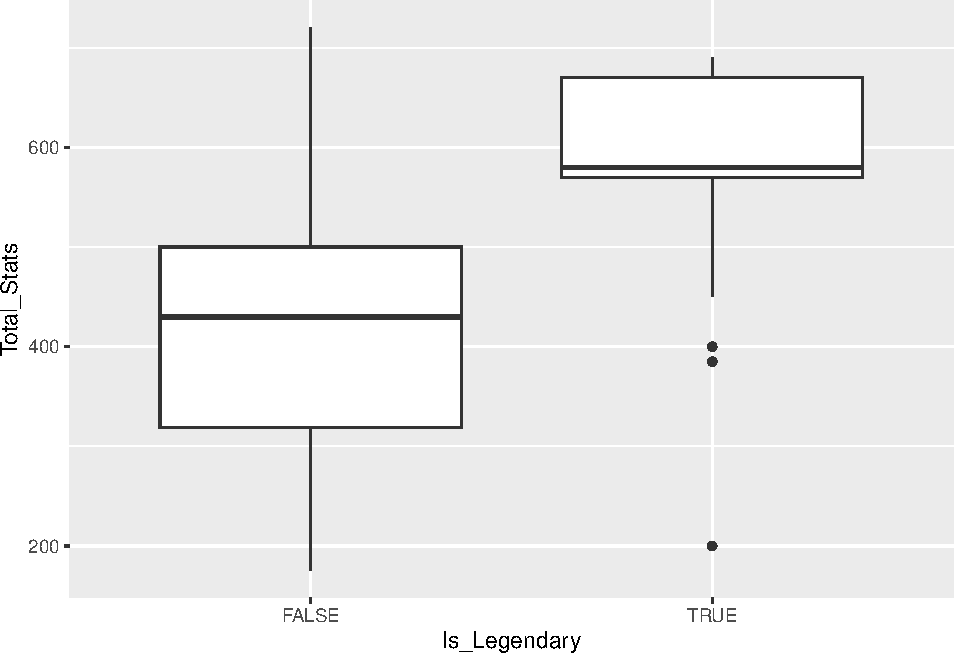
\includegraphics[width=0.9\linewidth,]{pokemon-statistical-analysis_files/figure-latex/unnamed-chunk-6-1} \end{center}

\end{document}
